%!TEX root = ../template.tex
%%%%%%%%%%%%%%%%%%%%%%%%%%%%%%%%%%%%%%%%%%%%%%%%%%%%%%%%%%%%%%%%%%%%
%% chapter3.tex
%% NOVA thesis document file
%%
%% This chapter includes a Literary Review.
%%%%%%%%%%%%%%%%%%%%%%%%%%%%%%%%%%%%%%%%%%%%%%%%%%%%%%%%%%%%%%%%%%%%
\chapter{Literature Review}
\label{cha:literature_review}

The work in this thesis involved dealing with many subjects. Air
Pollution, tomographic algorithms and DOAS (in particular DOAS
Tomography) were the most important. In this section, I provide a brief
literary review covering the three.

%%%%%%%%%%%%%%%%%%%%%%%%%%%%%%%%%%%%%%%%%%%%%%%%%%%%%%%%%%%%%%%%%%%%%%%%%%
%%%%%%%%%%%%%%%%%%%%%%%%%%%%%%%%%%%%%%%%%%%%%%%%%%%%%%%%%%%%%%%%%%%%%%%%%%
\section{Air pollution and pollutants}%
\label{sec:air_pollution_and_pollutants}

Daniel Vallero, in his book "Fundamentals of Air
Pollution"~\cite{Vallero2014} makes a very important observation: Air
Pollution has no universal definition. Its meaning is intertwined with
the context with which it is measured and observed, with the ecosystem
in which it is perceived and even with the pollutant concentration (not
every toxic compound is toxic at every concentration). The United States
Environmental Protection Agency (\gls{EPA}) defines Air Pollution as the
following:

\begin{center}
    \begin{minipage}{0.8\textwidth}

        \noindent
            \textit{Air Pollution is the presence of contaminants or pollutant
            substances in the air that interfere with human health or welfare,
            or produce other harmful environmental effects.}

    \end{minipage}
\end{center}

He then analyzes this definition through two possible lenses, the one
that comes with the interference produced by air contaminants; and the
one that comes from the harm they may cause. He notes that both points
of view come with a heavy burden of ambiguity, incompatible with a
scientific definition. We can thus observe that preferable to address
the issue through its measurable effects and consequences. These are
well-established and well known, and scientists all around the world
have been publishing extensively about them for some decades now. The
correlation between Air Pollution and an increased mortality in heavily
industrialized areas was first established in Europe, in the 19$^{th}$
century, but the first time it was taken seriously was during the 1952
killer-smog incidents, in London~\cite{Platt2007}. At the time, a
combination of very cold weather, an anticyclone and fireplace emissions
caused a thick smog to fall over London, directly causing thousands of
deaths and indirectly many more~\cite{Bell2008,Office2019}. The
disastrous consequences of this incident had a huge impact in the civil
society, resulting in a series of policies and laws, among which the
Clean Air Acts of 1956 and 1968.

More than 60 years have passed since the London-smog incident, but the
influence it had on the whole Western world has prevailed in time.
Almost every developed country in the world has laws and protocols in
place to limit and decrease \gls{AP} emissions over time. In the
European Union, the European Environmental Agency (\gls{EEA}) is
responsible for providing sound and independent information to the ones
involved developing, adopting, implementing and evaluating environmental
policy~\cite{EEA2019}. The agency is also responsible for publishing
reports on the state of air quality in Europe, which are made available
to the general public. In their most recent report~\cite{EEA2016}, one
could see that, in general, rules and regulations put in place to
control atmospheric emissions have caused a clear decreasing trend to
appear on \gls{AP} data (see Figure~\ref{fig:eu_chart_page}), although
European productivity has been rising or stable across all sectors.

\begin{figure}[htpb]
    \centering
    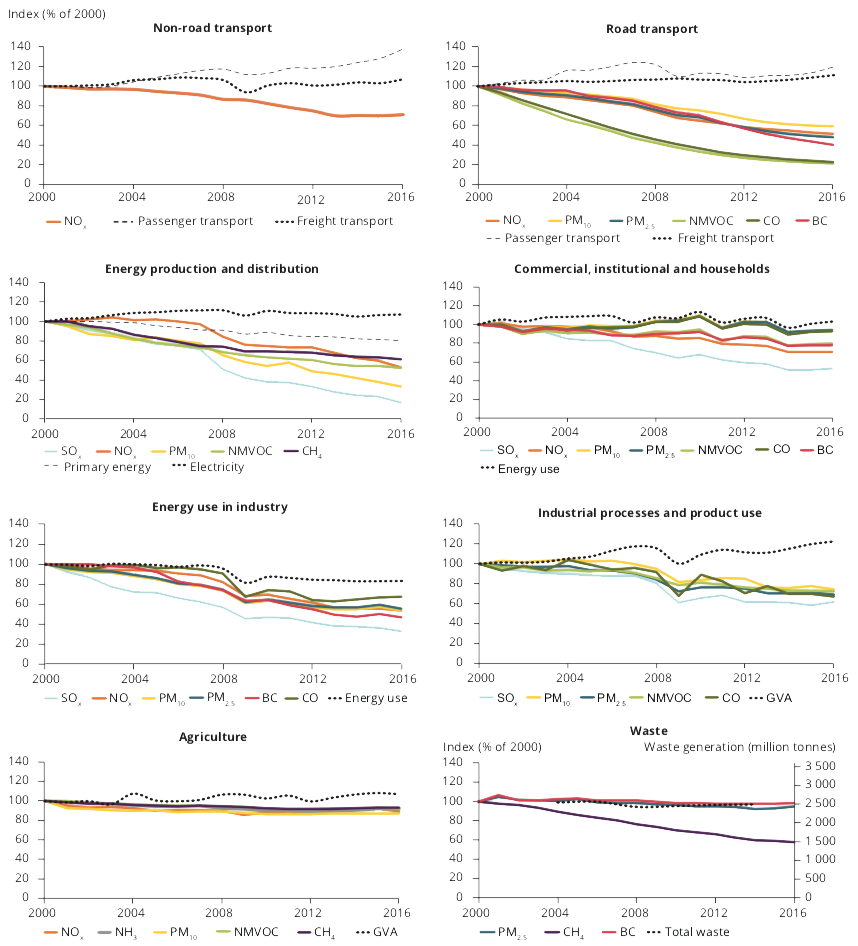
\includegraphics[width=\textwidth]{img/emissions.png}
    \caption{EU emissions evolution through time, since the year 2000,
    separated by source of emissions~\cite{EEA2016}. Notice the downward
    trend for emissions across all sources.}
    \label{fig:eu_chart_page}
\end{figure}

Reports like this one are very important in the current day Western
world. In fact, Europeans have deemed Air Pollution to be their second
largest environmental concern, after climate
change~\cite{TheEuropeanUnion2017}, with which it is inexorably
intertwined. The population's sensitivity to this subject is undoubtedly
related to the growing knowledge that exists regarding human health
implications of \gls{AP}. It has been known for some time that there is
a direct correlation between the emission level and premature mortality,
especially due to cardiovascular complications~\cite{Ghorani-Azam2016,
Carugno2016, Kampa2008, Kollanus2016}. In Europe, poor air quality is
an important cause of premature death, with a estimated toll of 400000
per year~\cite{EEA2016}.

A comprehensive description of the effects of Air Pollution on the human
and animal bodies would be a colossal task, much beyond the scope of
this document or my whole thesis. It is, however, important to mention
some of these effects, not only for demonstration purposes, but also as
an introductory approach to the physiological importance of \gls{AP},
which justify their social and societal significance as a public health
menace. I will therefore address the phenomenon impact on the
respiratory system, its importance as a precursor for cardiovascular
diseases and its potential impact on the most vulnerable period of human
life, gestation. The following discussion will once again be based
around Vallero's work~\cite{Vallero2014}, complemented whenever
necessary by other authors. 

The respiratory system's main functions are the delivery of oxygen into
the blood stream and the removal of carbon dioxide from the body. Air
enters the body from the upper airways and flows to the alveolar region,
where oxygen diffuses across the lung wall into the blood stream, from
which it is transported to the tissues where it diffuses yet again and
is made available to the mitochondria in the cells, that use it for
cellular respiration~\cite{Nilsson2010}. The whole system
is in permanent interaction with the atmosphere, and is therefore
exposed to all kinds of air pollutants and trace gases, increasing the
probability that some of them are delivered to this system. 

Acute symptoms of \gls{AP} exposure are very varied, and range from mild
irritation to complete respiratory failure, depending mostly on level of
exposure and individual sensitivity to the chemical compound. On a
chronic level, \gls{AP} has been established as cause for Chronic
Obstructive Pulmonary Disease (\gls{COPD}), asthma, and lung and other
cancers. In addition, by entering the body through the respiratory
system, air pollutants and toxins are conveyed onto the other tissues,
extending the range of their damage. The next system to be affected by
\gls{AP} is the cardiovascular system, which is the mechanism through
which the oxygen, absorbed by the respiratory system, gets transported
into all the other tissues. Oxygen is not the only molecule
that is able to traverse the lung's wall and therefore it is possible
for several air pollutants to contaminate the body through the same
paths. The link between Air Pollution and cardiovascular effects started
being made during the twentieth century, given a series of incidents
(like London's 1952 killer-smog) that happened in the urban areas of
industrialized countries. Nowadays, this link is perfectly established
and we have alredy described several mechanisms by which \gls{AP} is
able to interfere with cardiovascular health. For instance, scientists
and doctors have managed to establish at least three pathways between
\gls{AP} and cardiac arrhythmia, as depicted in
Figure~\ref{fig:arrhythmia}. One of the most important cardiovascular
complications that arise from Air Pollution is CO poisoning. Carbon
Monoxide is a tasteless, odorless and colorless gas that is a side
product from an incomplete combustion of fuels containing carbon atoms.
Its properties make it impossible to detect without some kind of
instrument, since our senses cannot distinguish its presence. CO can
easily enter the blood stream through the lungs. When in the body, it
binds with hemoglobin. Its affinity to this transport molecule is about
200 times higher than oxygen's, and this means that it starts to starve
the body organs from that important molecule. Continuous exposure to
Carbon Monoxide is never beneficial. Low exposure levels can cause
neuro-behavioral or developmental effects, but at higher concentrations,
the most prominent symptoms are unconsciousness and
death~\cite{Penney}.

\begin{figure}[htpb]
    \centering
    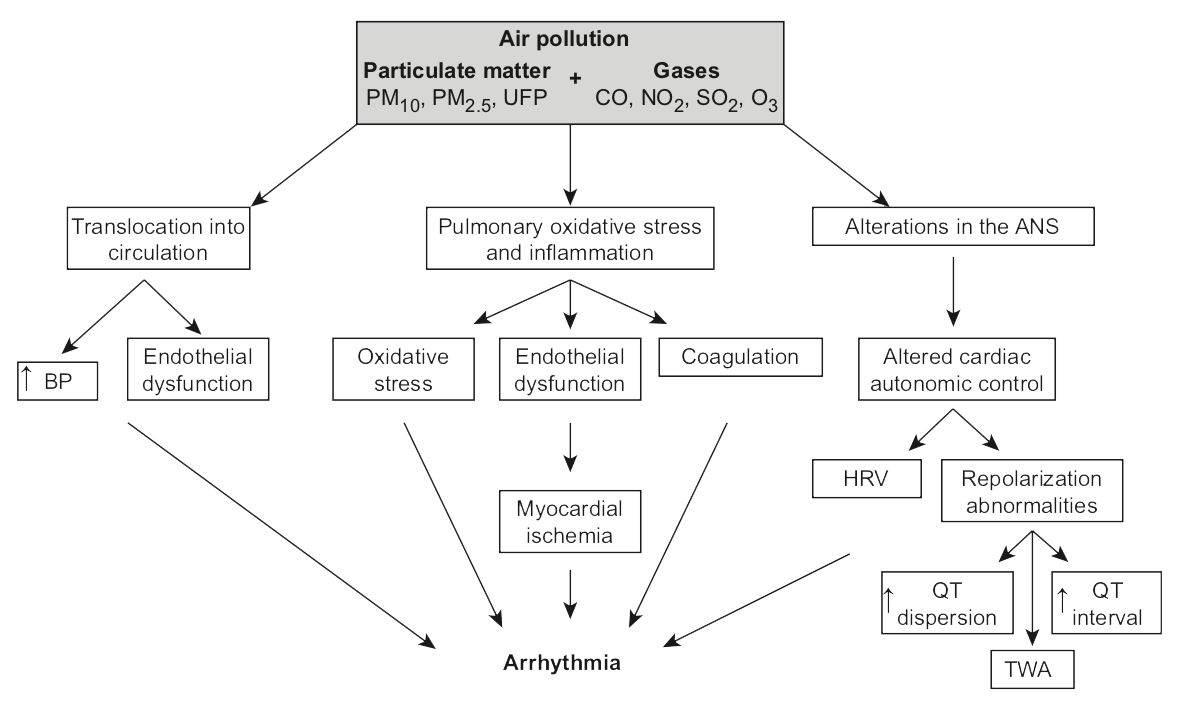
\includegraphics[width=0.8\textwidth]{img/arrhythmia.png}
    \caption{Physiological pathways to arrhythmia that stem from Air
    Pollution exposure~\cite{Vallero2014}.}
    \label{fig:arrhythmia}
\end{figure}

Mammals are in their life's most vulnerable stage while they are still
developing inside their mother's womb. This is the time when there is a
greater rate of tissue expansion and creation, which gives rise to the
possibility of the appearance of some kind of morphological abnormality.
This rate of development creates an enormous need for nutrients,
provided by the mother through her blood. If the mother is exposed to a
pollutant, and it gains access to the mother's blood stream, then the
developing being is also exposed. The effects that come from \emph{in
utero} exposure are similar to those we see in other stages of life, but
the dose at which they occur is significantly lower. Moreover, timing of
exposure is also important, since there are stages to the fetus'
development. Figure~\ref{fig:AP_in_utero}, taken
from~\cite{Vallero2014}, illustrates what kind of developmental effects
may come from Air Pollution exposure, and the influence of their timing.

\begin{figure}[htpb]
    \centering
    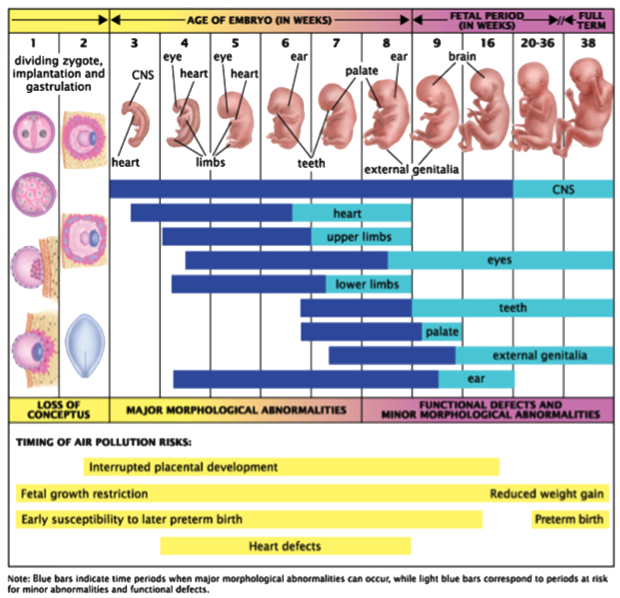
\includegraphics[width=0.8\textwidth]{img/development.png}
    \caption{Possible abnormalities caused by \gls{AP} exposure \emph{in
    utero}. Notice that time of exposure is of critical
    importance~\cite{Vallero2014}.}
    \label{fig:AP_in_utero}
\end{figure}

The seriousness of the effects these chemicals produce create the need
for quantification methods, so we can understand how we can deal with
our surrounding atmosphere. The variability of this our environment,
however, prevents the existence of any one-size-fits-all solution.  As a
result, there are many techniques and methods with which we are nowadays
able to measure pollution and airborne gaseous components. In the
following discussion, I will address only open path monitoring systems,
since these are the most relevant for the kind of project my thesis
encompasses. A more curious reader is redirected to ~\cite{Stewart1996,
Clark1997, Vallero2014} for a more in depth review and presentation of
emission monitoring technologies.

Open path atmospheric monitoring systems exploit interaction phenomena
between light and the gaseous pollutants to detect and measure pollutant
concentration. One of these technologies is Tunable Diode Laser
(\gls{TDL}), a technique in which light is emitted at a given wavelength
(particularly in the infrared region of the spectrum) and its
atmospheric absorption measured on the other end of the assembly.
\gls{TDL} has been used extensively for methane and NO measurements, and
provides robust results in real-time, being an adequate solution for
Continuous Emission Monitoring (\gls{CEM}). One of the greater
disadvantages of this technique is that, since only one wavelength is
measured at a time, one has to have a light source for each target
compound~\cite{Vallero2014, Bishop1996}. Another one of these techniques
is called Differential Absorption LIDAR (\gls{DIAL}). In this method,
light is pulsed in two different wavelengths, which must be close to one
another. The first of these wavelengths corresponds to an absorption
band of the substance in study, while the other is just off the
absorption peak. The ratio between the two received signals (one from
each emitted wavelengths) is proportional to the target pollutant
concentration~\cite{Stewart1996}. \gls{DIAL} technology allows
three-dimensional mapping of pollutant concentrations in a very flexible
and versatile way. It is many times used for mapping pollutant
concentration in urban settings. Its main drawbacks are the fact that it
is limited to a number of components and that \gls{DIAL} signals are
hard to analyze and can be contaminated by parasite chemical compounds,
which decrease the system's sensitivity to the intended pollutants.
Finally, we reach the most important open path monitoring technology in
this thesis, DOAS, which will be introduced in the next section, with
much more detail.

%%%%%%%%%%%%%%%%%%%%%%%%%%%%%%%%%%%%%%%%%%%%%%%%%%%%%%%%%%%%%%%%%%%%%%%%%%
%%%%%%%%%%%%%%%%%%%%%%%%%%%%%%%%%%%%%%%%%%%%%%%%%%%%%%%%%%%%%%%%%%%%%%%%%%
\section{DOAS}%
\label{sec:doas}

Differential Optical Absorption Spectroscopy is a well established
absorption technique that is widely used in the field of atmospheric
studies~\cite{Platt2007}. In this section, I present a short
introduction to the field, extracted from~\cite{ValentedeAlmeida2017},
an article we have published in 2017, marking the conclusion of the
initial studies for this PhD thesis.

There are two main families of \gls{DOAS} assemblies, with different
goals and capabilities:

\begin{itemize}

        \item Active systems, of which a simple illustration is
            presented in Fig.~\ref{fig:activeSmall}, are characterized
            by relying on an artificial light source for their
            measurements. A spectrometer at the end of the light path
            performs spectroscopic detection. Active DOAS techniques are
            very similar to traditional in-lab absorption spectroscopy
            techniques \cite{Platt2007};

        \item Passive DOAS techniques, illustrated in
            Fig.~\ref{fig:passiveSchematic}, use natural light sources,
            such as the Sun and the moon, in their measurement process.
            An optical system is pointed in certain elevation and
            azimuth angles and sends the captured light into a
            spectrometer, connected to a computer. The system returns
            the total value of the light absorption in its
            path~\cite{Platt2007,Merlaud2013}.

\end{itemize}

%f2
 \begin{figure*}[t]
    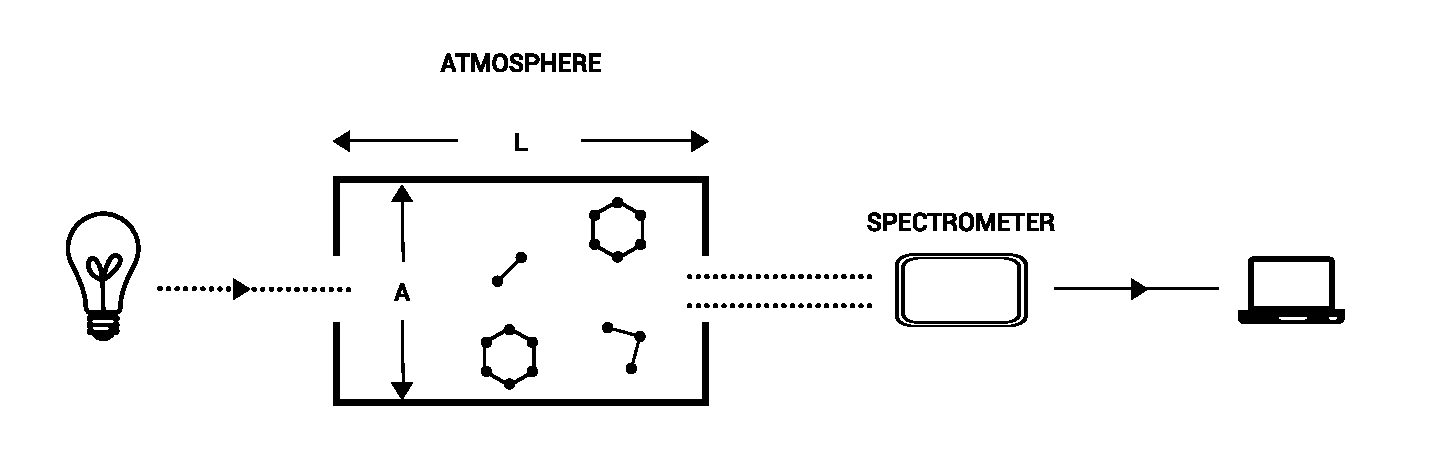
\includegraphics[width=14cm]{img/amt-2016-314-f02.pdf}
    \caption{Active DOAS schematic.}\label{fig:activeSmall}
  \end{figure*}

%f3
  \begin{figure*}[t]
      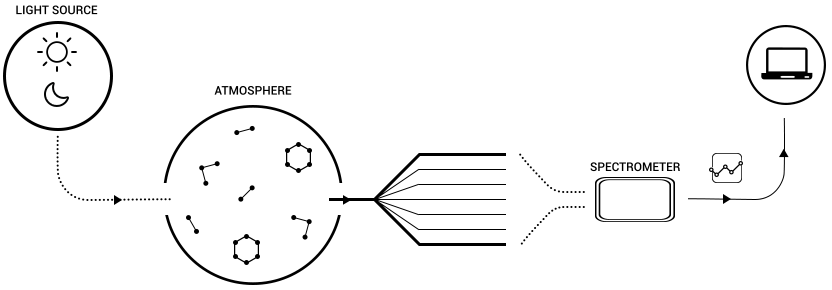
\includegraphics[width=14cm]{img/amt-2016-314-f03.png}
      \caption{Passive DOAS schematic.}\label{fig:passiveSchematic}
  \end{figure*}

DOAS itself is based on Lambert--Beer's law, which can be written as
\cite{Platt2007}

\begin{equation}
  \centering
  \label{eq:lambertBeer}
  I(\lambda) = I_0 (\lambda) \cdot \exp(-\sigma(\lambda) \cdot c \cdot L) \;,
\end{equation}

Where $\lambda$ is the wavelength of the emitted light; $I(\lambda)$ is
the light intensity as measured by the system; $I_{0}(\lambda)$ is the
intensity of the light as emitted by the source; and $\sigma(\lambda)$
is the absorption cross section of absorber, which is wavelength
dependent; $c$ is the concentration of the absorber we want to measure.


This law allows the definition of optical thickness
($\tau$)~\cite{Platt2007}:

\begin{equation}
      \label{eq:opticalThickness}
      \tau(\lambda) = \ln \bigg( \frac{I_{0}(\lambda)}{I(\lambda)}\bigg) = \sigma(\lambda) \cdot c \cdot
      L.
\end{equation}

In a laboratory setting, Eq.~(\ref{eq:lambertBeer})
or~(\ref{eq:opticalThickness}) can be used to directly calculate an
absorber's concentration, provided there is knowledge of  its cross
section. In the open atmosphere, however, absorption spectroscopy
techniques are far more complex. On one hand, $I_0(\lambda)$ is not
accessible since we measure from inside the medium we want to measure.
On the other hand, there are several environmental and instrumental
effects that influence measurement results. These effects include the
following~\cite{Platt2007}.

\begin{itemize}
      \item Rayleigh scattering is due to small molecules present in the
          atmosphere and is heavily influenced by wavelength (hence the
          blue colour of the
      sky).
      \item Mie scattering is caused by particles and larger molecules
          suspended in the atmosphere and is not very dependent
      on the wavelength (hence the white colour of clouds).
      \item Instrumental and turbulence effects are the instrument's
          transmissivity and atmospheric turbulence in the optical path
          also limit light intensity.

  \end{itemize}

In addition, we also have to take into account that, in the atmosphere,
there are a number of trace gases that interfere with passing light.

Another aspect worth mentioning is that our device is never pointed
directly at the light source (the Sun) but always processes light that
has been scattered at some unknown point in the optical path. This means
that the light that reaches our detector is only the scattered fraction
of the sunlight, depending on the system's position and geometry, as
well as wavelength.

The expansion of Lambert--Beer's equation to include all these effects
results in Eq.~(\ref{eq:expandedLambertBeer}).

\begin{align}
      \label{eq:expandedLambertBeer}
I(\lambda) & = I_{0}(\lambda) \cdot A(\lambda, \ldots) \cdot S(\lambda) \nonumber \\
      &\cdot
      \exp \Bigg[ - \int \Big[ \Big(\sum_{i} \sigma_{i}(\lambda, s) \cdot c_{i}(s)\Big) +
      \epsilon_\mathrm{M}(\lambda, s)\nonumber\\
      & + \epsilon_\mathrm{R}(\lambda, s) \Big]\mathrm{d}s \Bigg],
\end{align}

Where $A(\lambda, \ldots)$ is the fraction of scattered light that
reaches the device, $S(\lambda)$ represents instrumental and turbulence
effects, $\sigma_{i}(\lambda, s)$ is the absorption cross section of
absorber $i$, $c_{i}$ is the concentration of absorber $i$,
$\epsilon_\mathrm{R}(\lambda)$ represents Rayleigh's extinction
coefficient and $\epsilon_\mathrm{M}(\lambda)$ represents Mie's
extinction coefficient.


The interest of this equation lies within the retrieval of $c_i$, a
given absorber's concentration. Since the integral is taken along the
total atmospheric path of the measured photons, and considering that
their cross sections do not vary significantly in atmospheric
conditions, it is possible to define the concept of slant column, which
is of great importance~\cite{Merlaud2013}.

\begin{equation}
      \label{eq:slantColumn}
      \mathrm{SC}_{i} = \int c_{i}(s)\mathrm{d}s
\end{equation}

This quantity, as Eq.~(\ref{eq:slantColumn}) shows, equals the integral
of an individual absorber's concentration along the atmospheric optical
path of relevance.

Now, without knowledge of $I_{0}(\lambda)$, these equations cannot give
us absolute concentration values. We can, however, use another scattered
light spectrum as reference in Eq.~(\ref{eq:opticalThickness}). Instead
of absolute densities, this will yield relative changes in the
atmosphere. We thus arrive at Eq.~(\ref{eq:relativeOpticalThickness}).

\begin{align}
      \label{eq:relativeOpticalThickness}
      \ln\Big( \frac{I_\mathrm{ref}}{I}(\lambda) \Big) &= \ln\Big( \frac{A_\mathrm{ref}}{A}(\lambda,\ldots) \Big) + \ln\Big( \frac{S_\mathrm{ref}}{S}(\lambda) \Big) \nonumber\\
      &+  \sum_{i} (\sigma_{i}(\lambda) \cdot \Delta \mathrm{SC}_{i}(\lambda)) + \Delta \tau_\mathrm{M}(\lambda) \nonumber\\
      &+ \Delta \tau_\mathrm{R}(\lambda),
\end{align}

Where $\Delta \mathrm{SC}_{i}$  is the relative slant column of absorber
$i$; $\Delta \tau_\mathrm{M}$  is the relative Mie scattering term,
integrated to its optical thickness; and $\Delta \tau_\mathrm{R}$ is the
relative Rayleigh scattering term, integrated to its optical thickness.


This is where the principle of DOAS is applied. Instrument features,
scattering and other atmospheric effects have broad absorption spectral
profiles, which vary slowly with wavelength. Several trace absorbers
have narrow and rapidly varying spectral signatures in at least a small
section of the spectrum. By using Eq.~(\ref{eq:separation}), we can
separate these contributions \cite{Danckaert2015}.

\begin{equation}
      \label{eq:separation}
      \sigma(\lambda) = \sigma{'}(\lambda) + \sigma_{0}(\lambda)
\end{equation}

Here, the broad part of the optical thickness ($\sigma_{0}(\lambda)$)
can be separated from the narrow part ($\sigma{'}(\lambda)$ --
differential) by approximating it by a low-order polynomial, resulting
in Eq.~(\ref{eq:DOAS}).

\begin{equation}
      \label{eq:DOAS}
      \ln\Big( \frac{I_\mathrm{ref}}{I}(\lambda) \Big) = \sum_{i = 1}^{n} \sigma_{i}{'}(\lambda) \cdot \Delta \mathrm{SC}_{i} + \sum_{j = 0}^{m} a_{j} \cdot
      \lambda^{j},
\end{equation}

Where $\sum_{i = 1}^{n} \sigma_{i}{'}(\lambda) \cdot \Delta SC_{i}$ is
the differential part (narrowband, rapidly varying with wavelength) and
$\sum_{j = 0}^{m} a_{j} \cdot \lambda^{j}$ is a low-order polynomial,
used to remove the broadband spectral features resulting from
atmospheric and instrumental phenomena.


In practice, the mathematical solving of Eq.~(\ref{eq:DOAS}) is not
enough since it does not account for the Ring effect or the
non-linearities that result from stray light and wavelength shift in
measured and cross-section spectra.

The Ring effect is a consequence of rotational Raman scattering:
molecules in the atmosphere do not absorb photons in a purely elastic
(Rayleigh scattering) fashion. A small portion of the light--matter
interaction is in fact inelastic \cite{Brinkmann1968,Merlaud2013}. This
changes the light source frequencies as seen from the detector. This
phenomenon was first noticed by Grainger and Ring in 1962. At the time,
they noticed that the well-known Fraunhofer lines would slightly change
when one  observed them by using moonlight instead of scattered daylight
\cite{GRAINGER1962}.

From the occurrence of these phenomena, it results that the mathematical
procedure for DOAS measurements consists in solving a linear and a
non-linear problem. The linear problem is solved by writing
Eq.~(\ref{eq:DOAS}) in its matrix form:

\begin{equation}
      \label{eq:DOAS_matrix}
      \tau = \mathbf{A} \cdot X.
\end{equation}

$\mathbf{A}$ is an $m\,\times\,n$ matrix, with its columns being the
differential cross sections $\sigma_{i}{'}(\lambda)$ and the wavelength
powers taking the polynomial $P(\lambda) = \sum_{j = 0}^{m} a_{j} \cdot
\lambda^{j}$ into account. Since the number of lines in $A$ is much
larger than the number of columns, the system is overdetermined and, in
this case, we must use methods to numerically approximate a solution. It
is common to use the least-squares approach, in which the best solution
is the one that minimises $\chi^{2} = \left[\tau - A \cdot X\right]
\cdot \left[\tau - A \cdot X\right]^{T}$.

While the Ring effect is treated as a pseudo-absorber, a synthetically
produced~\cite{Chance1997} cross section that is fitted just like any
other absorber, non-linearities are addressed by applying
Levenberg--Marquardt's approach to non-linear fitting problems to
Eq.~(\ref{eq:DOAS_nonLinear}) \cite{Merlaud2013,Press2007}:


\begin{align}
      \label{eq:DOAS_nonLinear}
      &\ln\Big( \frac{I_\mathrm{ref}(\lambda)}{I(\lambda + \mathrm{shift}) + \mathrm{offset}} \Big) = \sum_{i = 1}^{n} \sigma_{i}{'}(\lambda) \cdot \Delta \mathrm{SC}_{i} \nonumber\\
      &+ \sum_{j = 0}^{m} a_{j} \cdot \lambda^{j},
\end{align}

Where shift and offset, which represent spectral wavelength shifts and
stray light offsets, respectively, are responsible for the non-linear
character of the problem.


%%%%%%%%%%%%%%%%%%%%%%%%%%%%%%%%%%%%%%%%%%%%%%%%%%%%%%%%%%%%%%%%%%%%%%%%%%
%%%%%%%%%%%%%%%%%%%%%%%%%%%%%%%%%%%%%%%%%%%%%%%%%%%%%%%%%%%%%%%%%%%%%%%%%%
\section{Tomographic algorithms and reconstruction techniques}%
\label{sec:tomographic_algorithms_and_reconstruction_techniques}

\subsection{Introduction}%
\label{sub:introduction}

Tomography is the cross-sectional imaging of an object through the use
of transmitted or reflected waves, captured by the object exposure to
the waves from a set of known angles. It has many different applications
in science, industry, and most prominently, medicine. Since the
invention of the Computed Tomography (\gls{CT}) machine in 1972, by
Hounsfield~\cite{Gunderman2006}, tomographic imaging techniques have had
a revolutionary impact, allowing doctors to see inside their patients,
without having to subject them to more invasive
procedures~\cite{Kak2001}.

Mathematical basis for tomography were set by Johannes Radon in 1917. At
the time, he postulated that  it is possible to represent a function
written in $\mathbb{R}$ in the space of straight lines, $\mathbb{L}$
through the function's line integrals. A line integral is an integral in
which the function that is being integrated is evaluated along a curved
path, a line. In the tomographic case, these line integrals represent a
measurement on a ray that traverses the Region Of Interest (\gls{ROI}).
Each set of line integrals, characterized by an incidence angle, is
called a projection (see Figure~\ref{fig:projection}). To perform a
tomographic reconstruction, the machine must take many projections
around the object. To the set of projections arranged in matrix form by
detector and projection angle, we call sinogram. All reconstruction
methods, analytical and iterative, revolve around going from reality to
sinogram to image~\cite{Bruyant2002, Kak2001, Herman1973, Herman1995,
Herman2009, Defrise2003}.

\begin{figure}[htpb]
    \centering
    
\includegraphics[width=0.5\textwidth]{img/projections.png}
    \caption{A schematic representation of a projection acquisition. In
    this image, taken from ~\cite{Herman2009}, the clear line that comes
    down at a diagonal angle is a projection.}
    \label{fig:projection}
\end{figure}

There are two broad algorithm families when it comes to tomographic
reconstruction, regarding the physics of the problem. The problem can
involve either non-diffracting sources (light travels in straight
lines), such as the X-Rays in a conventional \gls{CT} exam; or
diffracting sources, such as micro-waves or ultrasound in more
research-oriented applications~\cite{Kak2001}. In this document, I will
not address the latter family, since I will not be applying them in my
work. In the next few paragraphs, I will discuss the first family of
algorithms, and describe how an image can be reconstructed from an
object's projections when the radiation source is non-diffracting.

Let's consider the case in which we deal with a single ray of solar
light entering the atmosphere at a given point. Since the atmosphere
contains numerous absorbents and comparable atmospheric effects, the ray
changes from the point where it enters the atmosphere to the point at
which it is measured by a detector. Total absorption will depend on the
pollutant species, their cross-section and their concentration, since it
obeys Lambert-Beer's law. Looking from another angle, this absorption
is also the line integral that we will use to reconstruct our image.
With \gls{DOAS}, it is possible to measure several pollutants at the
same time, but for simplicity (and since it is one of the most studied
compounds in the field), let's consider that the single pollutant in our
atmospheric mixture is NO$_2$.

\subsection{Initial Considerations}%
\label{sub:initial_considerations}

The problem of tomographic reconstruction can be approached in a number
of ways, depending mostly on the authors. In my literary search, I have
found that Kak and Slaney~\cite{Kak2001} have certainly explained this
problem in one of the clearer ways available. Therefore, I shall base
the rest of my presentation in their writings, and complement with other
authors' notes wherever necessary.

Considering the coordinate system displayed in
Figure~\ref{fig:coordinates}. In this schematic, the object is
represented by the function $f(x, y)$. The  $(\theta, t)$ parameters can
be used to define any line in this schematic. Line AB in particular can
be written:

\begin{equation}
    \label{eq:lineAB}
    x \cdot \cos(\theta) + y \cdot \sin(\theta) = t
\end{equation}

\begin{figure}[htpb]
    \centering
    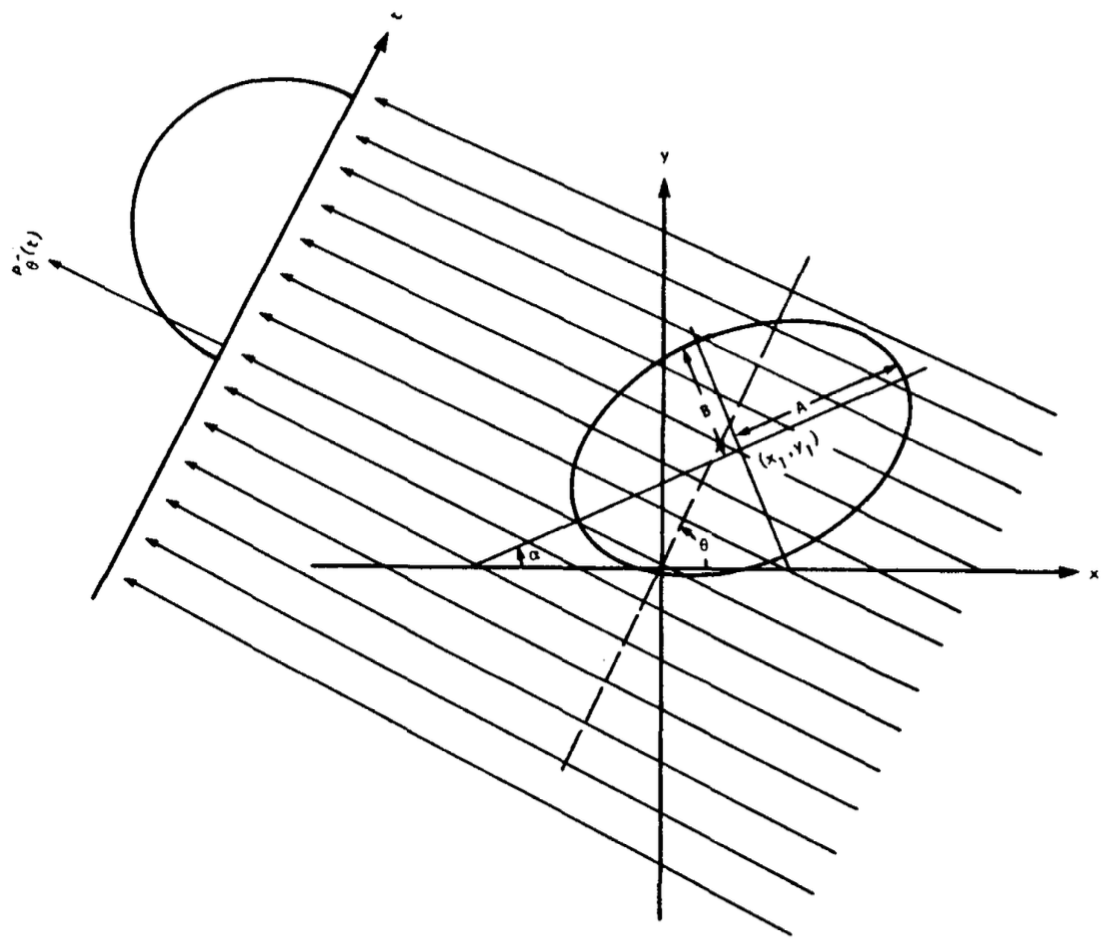
\includegraphics[width=0.7\textwidth]{img/coordinates.png}
    \caption{Schematic representation for coordinate setting.}
    \label{fig:coordinates}
\end{figure}

And if we were to write a line integral along this line, it would look
like Equation~\ref{eq:lineABIntegral}, the Radon transform of function
$f(x, y)$:

\begin{equation}
    \label{eq:lineABIntegral}
    P_{\theta}(t) = \int_{-\infty}^{\infty} f(x, y) \cdot \delta(x \cdot
    \cos(\theta) + y \cdot \sin(\theta) - t) dxdy
\end{equation}

Where $\delta$, the delta function, is defined in
Equation~\ref{eq:delta}.

\begin{equation}
    \label{eq:delta}
    \delta (\phi) =  
    \begin{cases}
            1, & \phi = 0\\
            0, & otherwise
    \end{cases}
\end{equation}

As I have mentioned previously, a projection is a set of line integrals
such as $P_{\theta}(t)$. Geometry plays a very important role in how the
integrals are written and solved for reconstruction. The simplest case
is the one where the set is acquired in a row, describing what is called
a parallel geometry. Another more complex case is when a single point
source is used as origin for all rays, forming a fan. This is called a
fanbeam array. There are other possible geometries, but they fall out of
the scope of this work and will therefore not be addressed any further.

\subsection{The Fourier Slice Theorem}%
\label{sub:the_fourier_slice_theorem}

The Fourier Slice Theorem (\gls{FST}) is the most important component of
the most important algorithm in tomographic inversion, the Filtered
BackProjection algorithm (\gls{FBP}). \gls{FST} is based on the equality
relation between the 
two-dimensional Fourier Transform (\gls{FT}) of the object function and
the one-dimensional \gls{FT} of the object's projection at an angle
$\theta$. Let's start by writing the 2D \gls{FT} for the object
function, Equation~\ref{eq:objectFT}, and the 1D \gls{FT} of projection
P$_\theta$, in Equation~\ref{eq:1dFTproj}.

\begin{equation}
    \label{eq:objectFT}
    F(u, v) = \int_{-\infty}^{\infty} \int_{-\infty}^{\infty} f(x, y)
    \cdot \exp \left [ -j2\pi (ux + vy) \right ] dx dy 
\end{equation}

\begin{equation}
    \label{eq:1dFTproj}
    S_{\theta}(\omega) = \int_{-\infty}^{\infty} P_{\theta} \cdot \exp\left[
    -j2 \pi \omega t \right]
\end{equation}

For simplicity, let's consider the 2D \gls{FT} at the line defined by
$v=0$ in the frequency domain. We rewrite the 2D \gls{FT} integral as:

\begin{equation}
    \label{eq:v0}
    F(u, 0) = \int_{-\infty}^{\infty} \int_{-\infty}^{\infty} f(x, y)
    \cdot \exp \left[  -j 2\pi  \omega ux \right] dx dy
\end{equation}

Notice that $y$ is not present in the phase factor of the \gls{FT}
expression anymore, and this means we can rearrange the integral as:

\begin{equation}
    \label{eq:v02}
    F(u, 0) = \int_{-\infty}^{\infty} \left[ \mathbf{\int_{-\infty}^{\infty}
    f(x, y) dy }\right] \cdot \exp \left[  -j 2\pi  \omega ux \right] dx 
\end{equation}

Now, the \textbf{bold} part of Equation~\ref{eq:v02} is similar to
Equation~\ref{eq:lineABIntegral}. It is precisely that equation,
considering $\theta=0$ and a constant value of $x$, as in
Equation~\ref{eq:p0}.

\begin{equation}
    \label{eq:p0}
    P_{\theta=0} (x) = \int_{-\infty}^{\infty} f(x, y) dy
\end{equation}

This in turn can be substituted in Equation~\ref{eq:v02}, finally
arriving at:

\begin{equation}
    \label{eq:FTP}
    F(u, 0) = \int_{-\infty}^{\infty} P_{\theta=0} (x) \cdot \exp \left[
    -j 2\pi ux \right] dx
\end{equation}

And this is the one-dimensional \gls{FT} for the projection at angle
$\theta=0$. Finally, the enunciation of the Fourier Slice Theorem:
\begin{center}
    \begin{minipage}{0.8\textwidth}

        \noindent\textbf{\emph{The Fourier Transform of a parallel
                projection  of an image $f(x, y)$ taken at angle
                $\theta$ gives a slice of the two-dimensional Fourier
                Transform, $F(u, v)$, subtending an angle $\theta$ with
                the $u$-axis (see Figure~\ref{fig:fst})}}

    \end{minipage}
\end{center}

\begin{figure}[htpb]
    \centering
    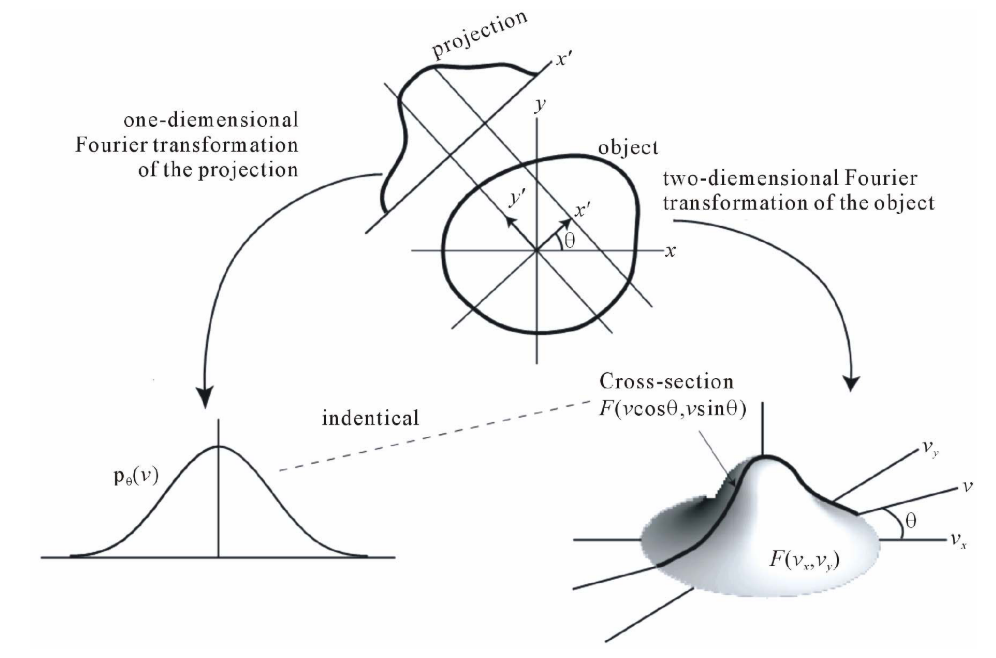
\includegraphics[width =.8\textwidth]{img/fst.png}    
    \caption{The \gls{FST}, a schematic representation.}
    \label{fig:fst}
\end{figure}

\subsection{The Filtered BackProjection Algorithm}%
\label{sub:the_filtered_backprojection_algorithm}

\subsubsection{The rationale for \gls{FBP}}%
\label{ssub:the_rationale_for_fbp}

If one takes the \gls{FST} into account, the idea behind the \gls{FBP}
seems to appear almost naturally. Say one has a single projection and
its Fourier transform. From the \gls{FST}, this projection is the same
as the object's two-dimensional \gls{FT} in a single line. A crude
reconstruction of the original object would result if someone were to
place this projection in its right place in the Fourier domain and then
perform a two-dimensional \gls{IFT}, while assuming every other
projection to be 0. The result, in the image space, would be as if
someone had smeared the object in the projections direction.

What is really needed for a correct reconstruction is to do this many
times, with many projections. This brings a problem with the method:
smearing the object in all directions will clearly produce a wrong
\emph{accumulation} in the center of the image, since every projection
passes through the middle (remember we are still talking about parallel
geometry projections) and are summed on top of each other, but on the
outer edges, this does not occur. If one does not address this, the
image intensity levels in the reconstructed image will be severely
overestimated in the center and underestimated in the edges (due to
normalization). The solution is conceptually easy: we multiply the
Fourier transform by a weighting filter proportional to its frequency
($\omega$) and that encompasses its relevance in the global scheme of
projections. If there are $K$ projections, then it is adequate for this
value to be $\frac{2\pi\lvert\omega\rvert}{K}$. As an algorithm,
\gls{FBP} can be written as in Algorithm~\ref{alg:fbp}.

\begin{algorithm}
    \caption{The Filtered BackProjection Algorithm}
    \label{alg:fbp}
    \begin{algorithmic}
        \FORALL{$\theta, \theta \in \left\{0..180,
        \frac{180}{K}\right\}$}
        \STATE{Measure projection $P_{\theta}(t)$;}
        \STATE{FT($P_{\theta}(t)$), rendering $S_{\theta}(\omega)$}
        \STATE{Multiply by $\frac{2\pi\lvert{\omega}\rvert}{K}$;}
        \STATE{Sum the \gls{IFT} of the result in the image space.}
    \ENDFOR
    \end{algorithmic}
\end{algorithm}

\subsubsection{Fan Projections Reconstruction}%
\label{ssub:fan_projections_reconstruction}

Parallel projections, in which the object is scanned linearly from
multiple directions, have the advantage of having a relatively simple
reconstruction scheme. However, they usually result in acquisition times
which are in the order of minutes. A faster way of collecting the data
is one where all radiation emanates from a single point-source, which
rotates around the target object (as well as the detectors). There are
two types of fan beam projections: equiangular and equally spaced. In
this project, I have only worked with equiangular processes, so I will
not include an explanation for equally spaced fan beam projections. The
reader may find this well described (much better than I would be able
to) in ~\cite{Kak2001} and ~\cite{Herman1973}.

Consider Figure~\ref{fig:equiangular}. If our projection data were
acquired through a parallel ray geometry, we would be able to say that
ray SA belonged to a projection $P_{\theta}(t)$, in which $\theta$ and
$t$ would be written:

\begin{equation}
    \label{eq:theta_and_t}
    \theta = \beta + \gamma \quad \text{ and } \quad t = D \cdot \sin \gamma
\end{equation}

In Equation~\ref{eq:theta_and_t}, $D$ is the distance between the source
$S$ and the origin $O$; $\gamma$ is the angle of a ray within a fan and
$\beta$ is the angle that the source $S$ makes with a reference axis.

\begin{figure}[htpb]
    \centering
    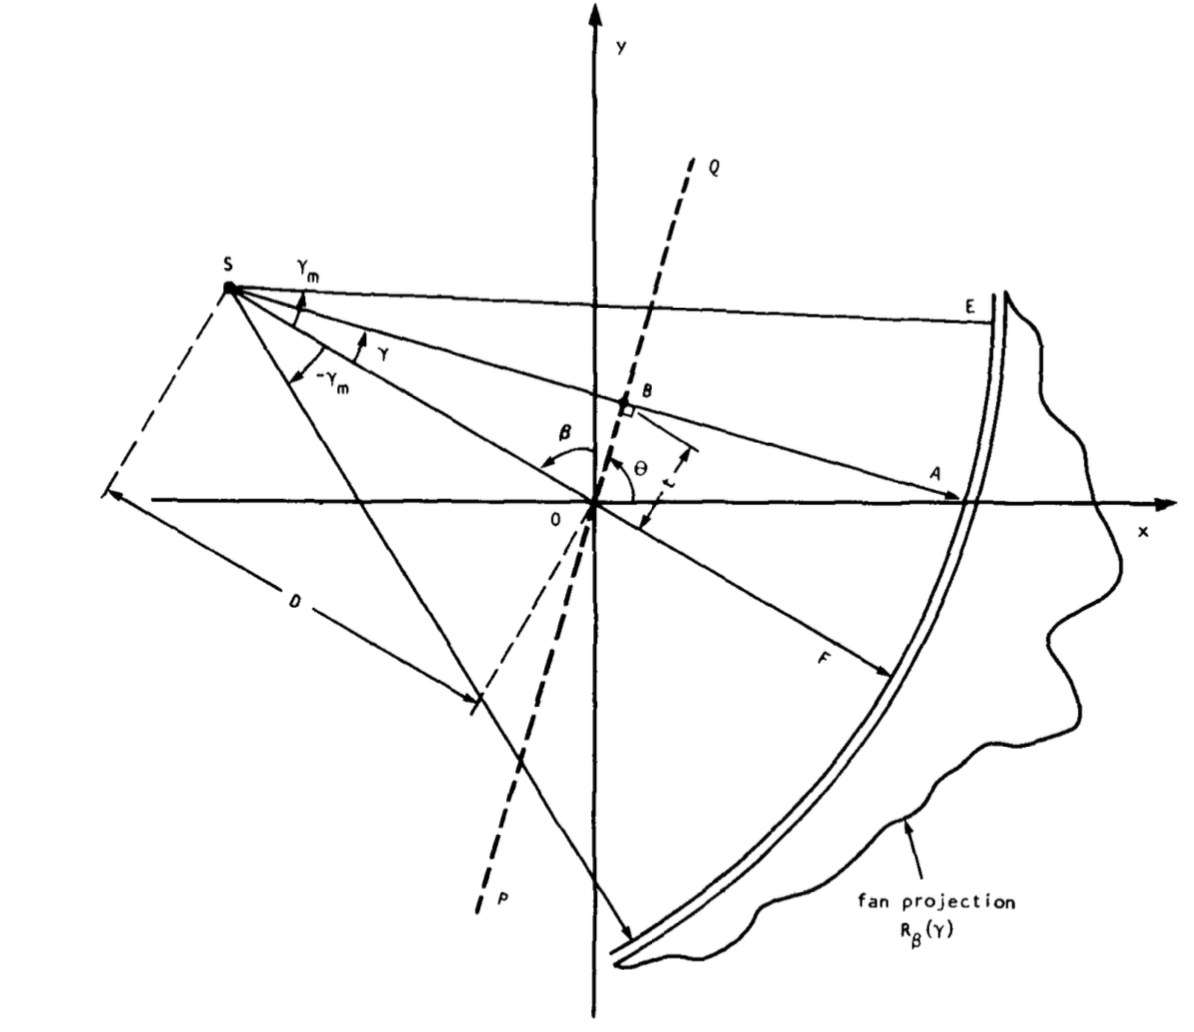
\includegraphics[width=.8\textwidth]{img/fig319.png}
    \caption{Schematic representation of an equiangular fan beam
    projection, taken from~\cite{Kak2001}.}
    \label{fig:equiangular}
\end{figure}


%%%%%%%%%%%%%%%%%%%%%%%%%%%%%%%%%%%%%%%%%%%%%%%%%%%%%%%%%%%%%%%%%%%%%%%%%%
%%%%%%%%%%%%%%%%%%%%%%%%%%%%%%%%%%%%%%%%%%%%%%%%%%%%%%%%%%%%%%%%%%%%%%%%%%
\section{DOAS tomography}%
\label{sec:doas_tomography}

During the course of this project, I wrote a Systematic Mapping Study
(\gls{SMS}) on DOAS tomography. The purpose of this study was to find
the current state of affairs regarding DOAS Tomography in the
literature. To avoid repetition, this article was included in full in
Appendix~\ref{ap:tomDoas}.

%%%%%%%%%%%%%%%%%%%%%%%%%%%%%%%%%%%%%%%%%%%%%%%%%%%%%%%%%%%%%%%%%%%%%%%%%%
%%%%%%%%%%%%%%%%%%%%%%%%%%%%%%%%%%%%%%%%%%%%%%%%%%%%%%%%%%%%%%%%%%%%%%%%%%

